\documentclass[11pt,a4paper]{article}

\usepackage[margin=1in]{geometry}
\usepackage{graphicx}
\usepackage{float}
\usepackage{amsmath}
\usepackage[utf8]{inputenc}
\usepackage[T1]{fontenc}
\usepackage{lmodern}
\usepackage{microtype}
\usepackage{csquotes}
\usepackage[english]{babel}
\usepackage{cite}
\usepackage{listings}
\usepackage{xcolor}
\usepackage{caption,subcaption}
\usepackage{booktabs}
\usepackage[hidelinks]{hyperref}

\lstset{
    basicstyle=\ttfamily\small,
    keywordstyle=\color{blue},
    commentstyle=\color{gray},
    breaklines=true
}
 
\makeatletter
% allow a subtitle
\providecommand\@subtitle{}
\newcommand{\subtitle}[1]{\gdef\@subtitle{#1}}

% provide a way to set two author emails
\providecommand\@emailone{email1@example.com}
\providecommand\@emailtwo{email2@example.com}
\newcommand{\authoremails}[2]{\gdef\@emailone{#1}\gdef\@emailtwo{#2}}

% default subtitle and emails (editable)
\subtitle{Máster en Inteligencia Artificial - Universidad de Murcia}
\authoremails{jdiego.gallego@um.es}{oscar.veral@um.es}

% Redefine \maketitle to produce a dedicated titlepage
\renewcommand{\maketitle}{%
    \begin{titlepage}
        \centering
        \thispagestyle{empty}
        \vspace*{2.5cm}
        {\Huge\bfseries\@title\par}
        \vspace{1cm}
        {\Large\itshape\@subtitle\par}
        \vspace{3cm}
        {\large
            \begin{tabular}{c}
                \@author
            \end{tabular}\par
        }
        \vspace{0.6cm}
        {\small
            \begin{tabular}{c}
                \texttt{\@emailone} \\[0.8ex]
                \texttt{\@emailtwo}
            \end{tabular}\par
        }
        \vfill
        {\large \@date\par}
    \end{titlepage}%
}
\makeatother

\begin{document}

\title{Informe BT5\\[1ex]\large Visión Artificial}
\author{Juan Diego Gallego Nicolás \and Óscar Vera López}
\date{\today}

\maketitle

\renewcommand{\contentsname}{Índice}
\setcounter{tocdepth}{3}
\tableofcontents
\clearpage


\section*{Introducción}
En este informe se detallan las implementaciones y resultados obtenidos en las tareas de procesamiento de imágenes realizadas para el bloque de trabajo BT5.

\section*{Items cubiertos}
\begin{itemize}
    \item \textbf{BT5c}: Calibración interínseca (tablero, Charuco o autocalibración simple).
    \item \textbf{BT5e}: Realidad aumentada mínima.
    \item \textbf{BT5i}: Detección con precisión subpíxel.
    \item \textbf{BT5m}: Video rectificación/estabilización por homografía.
\end{itemize}

\clearpage

\section{BT5: Geometría proyectiva, calibración y realidad aumentada}

En esta sección se describen las tareas realizadas para el bloque de trabajo BT5, centrado en la calibración de cámaras y la aplicación de realidad aumentada
usando geometría proyectiva. El ámbito del proyecto cambia totalmente con respecto al de los bloques anteriores, centrándonos en este caso en 
la creación de una aplicación de realidad aumentada para jugar al ajedrez.

La realidad aumentada (RA o AR por sus siglas en inglés) combina elementos visuales generados por un ordenador con el entorno físico en tiempo real.
Para llevar a cabo esta proyección, es necesario conocer el modelo físico de la cámara que captura el entorno, lo cual se consigue mediante un proceso de calibración.
Una vez calibrada la cámara, se puede utilizar la información obtenida para estimar la pose de la plantilla de referencia y proyectar objetos 3D en la escena, alineándolos correctamente con el mundo real.
En nuestro caso usaremos un tablero de ajedrez físico como marcador plano para calibrar la cámara y superponer las piezas de ajedrez en sus posiciones correspondientes.
Las piezas han sido modeladas como perfiles de revolución y se renderizan con un modelo de iluminación simple para dar sensación de volumen.

\subsection{Detección del tablero y calibración}

Para superponer objetos virtuales sobre el mundo real 
el primer paso es detectar un patrón conocido que sirva como 
sistema de referencia. Se ha utilizado un tablero de ajedrez 
estándar de $7 \times 7$ esquinas internas ($8 \times 8$ cuadros)
y el algoritmo de detección de esquinas de OpenCV. La implementación se encuentra en la función \texttt{dectect\_board} del módulo \texttt{detection.py}.

\subsubsection{Detección y refinamiento}
El algoritmo de detección implementado en la función \texttt{dectect\_board} sigue una serie de pasos optimizados para garantizar el rendimiento en tiempo real:

\begin{enumerate}
    \item \textbf{Preprocesamiento:} La imagen de entrada se convierte a escala de grises para simplificar el análisis de gradientes.
    
    \item \textbf{Optimización por Escala:} Dado que elegimos procesar imágenes de alta resolución (1280x720) y que
    el método \texttt{findChessboardCorners} de OpenCV es lento descartando imágenes en las que no encuentra el patrón,
    implementamos una optimización piramidal. Primero se redimensiona la imagen a un factor de $0.3$. 
    Si la función \texttt{findChessboardCorners} no detecta el patrón en esta versión reducida (usando el flag \texttt{CALIB\_CB\_FAST\_CHECK}), 
    se descarta el frame inmediatamente, ahorrando tiempo de cómputo. Solo si la detección preliminar es 
    positiva se procede a buscar en la imagen original.
    
    \item \textbf{Refinamiento Sub-píxel:} La detección inicial devuelve 
    coordenadas enteras de los píxeles. Para evitar el "temblor" (jitter) en los objetos 3D, 
    es crítico obtener una precisión sub-píxel. Se aplica \texttt{cv2.cornerSubPix} con un 
    criterio de parada basado en una tolerancia y número de iteraciones.
\end{enumerate}

\textit{\textbf{BT5c, BT5i}}

\subsubsection{Estabilización del sistema de coordenadas}
Uno de los mayores desafíos al usar marcadores cuadrados simétricos es la ambigüedad rotacional. 
El detector estándar de OpenCV puede devolver las esquinas en órdenes diferentes (rotadas 90º, 180º o transpuestas) 
dependiendo de la iluminación o el ángulo de la cámara, lo que causaría 
que el sistema de coordenadas virtual "saltase" erráticamente.

Para solucionar esto, se implementaron dos estrategias de ordenación en las funciones \texttt{sort\_corners} y \texttt{sort\_corners\_hist}:

\begin{itemize}
    \item \textbf{Heurística Geométrica:} En ausencia de información previa, 
    el sistema analiza los vectores que forman la primera fila y columna del grid detectado. 
    Se aplican transformaciones (transposición y espejos) para forzar matemáticamente que el 
    vector $(0,0) \to (0,1)$ apunte hacia la derecha de la imagen (Eje X) y el vector $(0,0) \to (1,0)$ 
    apunte hacia abajo (Eje Y). Esto no resulta relevante para la calibración inicial, pero
    sí para mantener una orientación consistente en la proyección 3D. La heurística utilizada es:
    ubicar la esquina superior izquierda del tablero lo más cerca posible del origen de coordenadas de la imagen (0,0), 
    que será la esquina a la derecha del jugador negro (A8).
    
    \item \textbf{Coherencia Temporal:} Para permitir movimientos orbitales de 360º alrededor 
    del tablero sin inversiones de ejes, se utiliza la información del frame anterior (\texttt{prev\_corners}). 
    El algoritmo genera las 8 permutaciones posibles (rotaciones y espejos) de las nuevas esquinas detectadas 
    y selecciona aquella que minimiza la distancia Euclídea respecto a las esquinas del frame anterior. 
    Esto garantiza una transición suave y coherente en la orientación del sistema de coordenadas entre frames consecutivos.
\end{itemize}

\textit{\textbf{BT5m}}

\subsubsection{Calibración Intrínseca}
Para obtener los parámetros intrínsecos de la cámara desarrollamos un pequeño script interactivo que permite al 
usuario capturar múltiples vistas del tablero desde diferentes ángulos. Cada vez que se desee, pulsando la tecla 
\texttt{'s'}, se captura la imagen actual siempre que el patrón haya sido detectado correctamente. Al pulsar 
\texttt{'c'} y teniendo al menos 10 vistas capturadas, se procede a la calibración. En la Figura \ref{fig:calib_gui} se muestra la interfaz gráfica del proceso.

\begin{figure}[H]
    \centering
    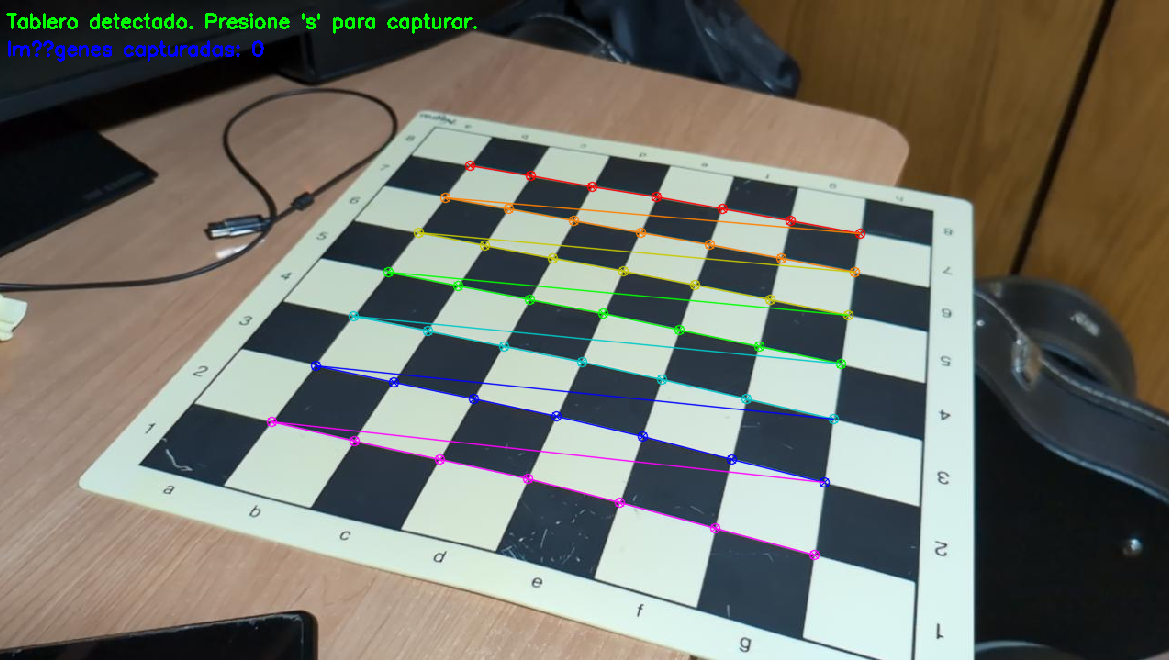
\includegraphics[width=0.6\textwidth]{images/calib_gui.png}
    \caption{Interfaz gráfica para la captura de vistas y calibración de la cámara.}
    \label{fig:calib_gui}
\end{figure}

Utilizando el método de Zhang implementado en \texttt{cv2.calibrateCamera} 
se resuelve el sistema de ecuaciones que relaciona las correspondencias entre los puntos 3D del mundo real (definidos con $Z=0$) 
y los puntos 2D detectados. El resultado es la matriz de cámara $K$ y los coeficientes de distorsión, 
que se almacenan en un archivo \texttt{.npz} para su carga posterior.

\begin{equation}
K = \begin{bmatrix} 
f_x & 0 & c_x \\ 
0 & f_y & c_y \\ 
0 & 0 & 1 
\end{bmatrix} 
= 
\begin{bmatrix} 
1093.04 & 0 & 620.03 \\ 
0 & 1069.09 & 308.74 \\ 
0 & 0 & 1 
\end{bmatrix}
\end{equation}

Se observa que el centro óptico $(c_x, c_y) = (620.03, 308.74)$ se encuentra razonablemente cerca del centro geométrico de la imagen $(640, 360)$, lo cual es consistente con una óptica estándar.

Por último, los coeficientes de distorsión radial y tangencial ($k_1, k_2, p_1, p_2, k_3$) calculados son:

\begin{equation}
D = \begin{bmatrix} 
0.3861 & -2.8986 & 0.0048 & -0.0066 & 6.4662 
\end{bmatrix}
\end{equation} 

\subsection{Modelado de piezas de ajedrez}

A excepción del caballo, todas las piezas de un juego de ajedrez clásico presentan simetría de revolución (obviando algunos detalles). Por ello, hemos optado por modelar las piezas definiendo su perfil 2D en el plano XZ y rotándolo alrededor del eje Z. \\

\textbf{Nota de diseño:} debido a que la geometría del caballo no presenta simetría rotacional y su modelado mediante revolución es inviable, hemos optado 
por sustituirlo por un modelo con forma de espada que sí puede ser modelado mediante revolución.
\\

La definición de los perfiles se almacena en la carpeta \texttt{resources/assets} como archivos de texto plano. 
Cada línea de estos archivos contiene las coordenadas $X,Z$ de vértices del perfil separados por comas.
Todos los diseños han sido realizados manualmente por los autores usando como referencia un juego de ajedrez físico y la herramienta 
de matemática gráfica \textit{GeoGebra}. En la siguiente imagen 
se muestra el perfil de la reina y su correspondiente modelo 3D generado.

\begin{figure}[H]
    \centering
    \begin{subfigure}{0.4\textwidth}
        \centering
        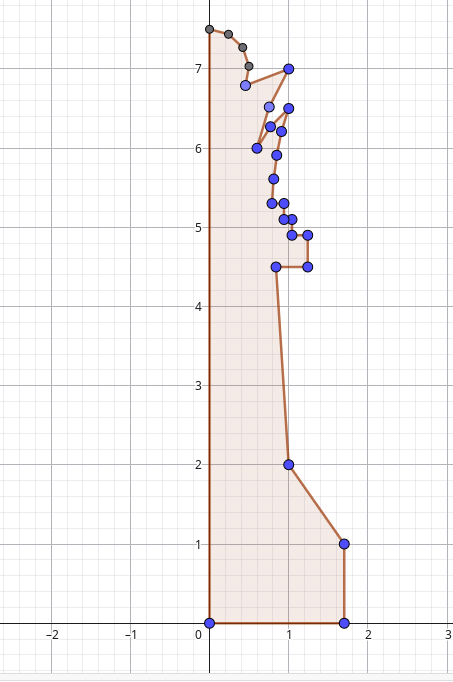
\includegraphics[width=0.8\textwidth]{images/queen_profile.png}
        \caption{Perfil 2D de la reina.}
    \end{subfigure}
    \hfill
    \begin{subfigure}{0.4\textwidth}
        \centering
        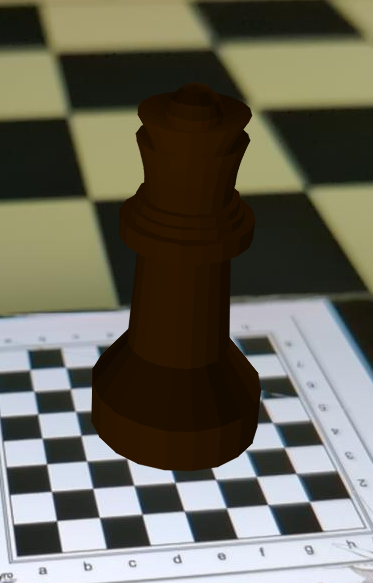
\includegraphics[width=0.8\textwidth]{images/queen.png}
        \caption{Modelo 3D generado por revolución.}
    \end{subfigure}
    \caption{Modelado de la pieza de la reina mediante perfil y revolución.}
    \label{fig:queen_model}
\end{figure}

La malla 3D se genera rotando el perfil $N$ veces alrededor del ejer $Z$. Las coordenadas de los vértices generados siguen la ecuación paramétrica:
\begin{equation}
\begin{cases}
x_{i,j} = r_i \cdot \cos(\theta_j) \\
y_{i,j} = r_i \cdot \sin(\theta_j) \\
z_{i,j} = -z_i \quad (\text{Invertido para sistema de cámara})
\end{cases}
\end{equation}

Donde $\theta_j = \frac{2\pi j}{N}$. En nuestro caso utilizamos $N=20$ para mostrar las 
piezas en detalle y $N=12$ para el renderizado en tiempo real.

\subsection{Motor de renderizado}

En versiones preliminares del proyecto, la proyección de las piezas resultó ser un cuello
de botella significativo, ya que una resolución de 12 rotaciones implica procesar más de 7600 triángulos por fotograma.
Para alcanzar una tasa de frames adecuada ($\approx$30 FPS), se ha implementado un motor de renderizado personalizado optimizado para nuestro caso de uso específico.

\subsubsection{Transformación de coordenadas}

Para cada pieza, primero se trasladan y rotan sus vertices a su posición en el tablero.
Posteriormente, se proyectan los vértices 3D a coordenadas 2D de imagen usando la pose estimada del tablero:

\begin{equation}
P_{cam} = R \cdot P_{world} + t
\end{equation}

Esta operación se realiza de forma vectorizada usando NumPy para maximizar la eficiencia.

\subsubsection{Iluminación y ocultación}

Para dotar de volumen a las piezas y evitar dibujar caras innecesarias, para cada triángulo de la malla se hace lo siguiente:
\begin{itemize}
    \item \textbf{Cálculo de normales:} Para cada triángulo definido por los vértices $A, B, C$ se calcula el vector normal $\vec{n}=\frac{(B-A) \times (C-A)}{\|(B-A) \times (C-A)\|}$. Es importante mantener la orientación consistente de las normales y garantizar que los vértices constituyan una cara.
    \item \textbf{Determinación de visibilidad:} Se calcula el producto escalar entre la normal y el vector que une el centro de la cámara con el centro del triángulo. Dependiendo se la definición del vector normal, el resultado será un valor positivo o negativo según la cara esté orientada hacia la cámara (visible) o no (oculta).
    En nuestro caso, si el valor es positivo, la cara es visible.
    \item \textbf{Cálculo de iluminación:} Para las caras visibles, se calcula la intensidad de iluminación usando un modelo de iluminación difusa simple (Lambertiano). Se define una fuente de luz direccional fija y se calcula la intensidad como $I=0.4+0.6\times |\vec{n}\cdot\vec{L}|$
\end{itemize}

\subsubsection{Ordenación}

Para resolver el problema de la oclusión entre piezas y caras de una misma pieza, adaptamos el algortimo del pintor (painter's algorithm).
Se calcula la profundidad media de cada cara visible y se ordenan de mayor a menor profundidad. Esto garantiza que las caras más alejadas se dibujen primero, 
permitiendo que las caras más cercanas las tapen correctamente. Las caras se dibujan usando la función \texttt{cv2.fillConvexPoly} de OpenCV,
aplicando el color calculado en el paso de iluminación.

Gracias a estas optimizaciones, el proceso de renderizado se ha reducido de más de 300 ms en versiones preliminares
a aproximadamente 30 ms en un ordenador con CPU AMD Ryzen 7 5800H, permitiendo alcanzar tasas de frames adecuadas para una experiencia fluida de realidad aumentada.

% Insertar grid 3x2 de las piezas renderizadas
\begin{figure}[H]
    \centering
    \begin{subfigure}{0.3\textwidth}
        \centering
        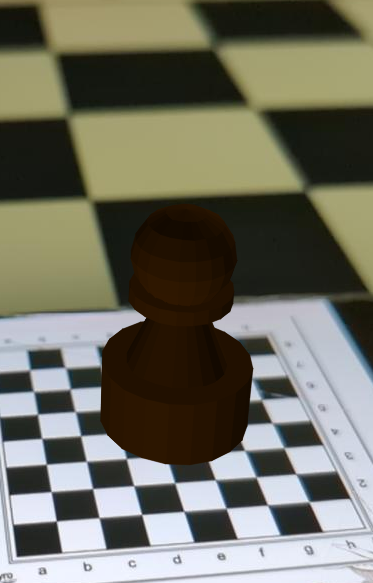
\includegraphics[width=0.8\textwidth]{images/pawn.png}
        \caption{Peón}
    \end{subfigure}
    \hfill
    \begin{subfigure}{0.3\textwidth}
        \centering
        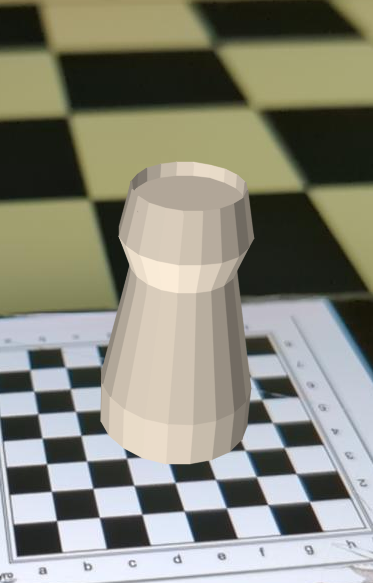
\includegraphics[width=0.8\textwidth]{images/rook.png}
        \caption{Torre}
    \end{subfigure}
    \hfill
    \begin{subfigure}{0.3\textwidth}
        \centering
        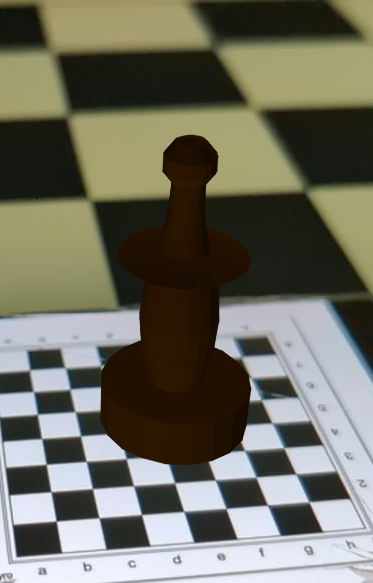
\includegraphics[width=0.8\textwidth]{images/knight.png}
        \caption{Caballo}
    \end{subfigure}
    \vfill
    \begin{subfigure}{0.3\textwidth}
        \centering
        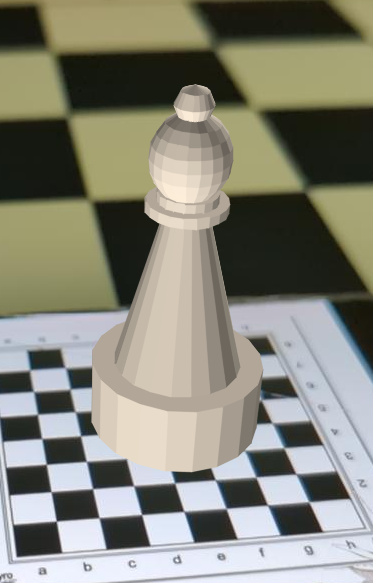
\includegraphics[width=0.8\textwidth]{images/bishop.png}
        \caption{Alfil}
    \end{subfigure}
    \hfill
    \begin{subfigure}{0.3\textwidth}
        \centering
        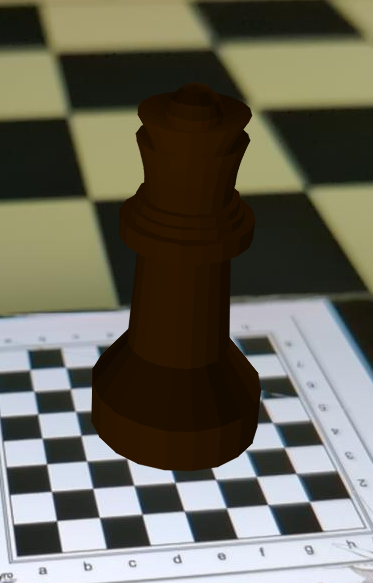
\includegraphics[width=0.8\textwidth]{images/queen.png}
        \caption{Reina}
    \end{subfigure}
    \hfill
    \begin{subfigure}{0.3\textwidth}
        \centering
        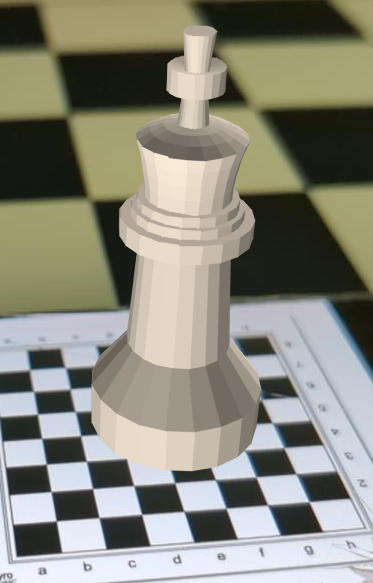
\includegraphics[width=0.8\textwidth]{images/king.png}
        \caption{Rey}
    \end{subfigure}
    \caption{Piezas de ajedrez renderizadas en 3D mediante el motor personalizado.}
    \label{fig:chess_pieces}
\end{figure}

\textit{\textbf{BT5e}}

\subsection{Integración del sistema y aplicación Final}

El script principal (\texttt{main.py}) integranda los módulos de visión por computador, la lógica de ajedrez (mediante la librería \texttt{python-chess}) y el motor de renderizado en un bucle de ejecución en tiempo real. A continuación se detallan los componentes clave de la arquitectura final.

\subsubsection{Gestión de configuración}

Para evitar la codificación rígida (\textit{hardcoding}) de parámetros y facilitar la portabilidad del sistema entre diferentes equipos y cámaras, se ha implementado un sistema de configuración basado en archivos YAML.
El sistema carga al inicio parámetros críticos como:
\begin{itemize}
    \item \textbf{Cámara:} Índice del dispositivo, resolución deseada y ruta al archivo de calibración \texttt{.npz}.
    \item \textbf{Juego:} Factor de escala para el tamaño de las piezas. Con $scale=1.0$ las piezas se muestran con un tamaño realista dentro de su casilla. Disminuir este parámetro aumenta la proporción pieza/tablero, pudiendo verse estas en más detalle.
    \item \textbf{Rutas:} Ubicación de los perfiles de las piezas y directorio de partidas guardadas.
\end{itemize}

\subsubsection{Bucle de Realidad Aumentada}

El núcleo de la aplicación es un bucle infinito que procesa el flujo de vídeo frame a frame. La lógica de control sigue una máquina de estados secuencial:

\begin{enumerate}
    \item \textbf{Adquisición y detección:} Se captura el frame y se busca el tablero utilizando la función optimizada \texttt{detect\_board}, aprovechando la coherencia temporal del frame anterior.
    
    \item \textbf{Estimación de pose (PnP):} Si se detecta el tablero, se resuelve la perspectiva para obtener los vectores de rotación ($r_{vec}$) y traslación ($t_{vec}$).
    
    \item \textbf{Persistencia:} Se ha implementado un contador de pérdida de tracking. Si el tablero no se detecta en un frame, el sistema continúa usando la última pose
    conocida durante 8 frames antes de considerar que se ha perdido.
    Esto se combina con un filtro temporal para suavizar la pose, de forma que las piezas no "salten" erráticamente entre recuperaciones:
    \begin{equation}
    v_{t} = \alpha \cdot v_{t-1} + (1 - \alpha) \cdot v_{new}
    \end{equation}
    En nuestra implementación, utilizamos un factor de suavizado $\alpha = 0.6$. Este efecto se verá con más claridad en el vídeo adjunto.
\end{enumerate}

\subsubsection{Interfaz de usuario e interactividad}

Para convertir la demostración técnica en una aplicación utilizable, se ha desarrollado una interfaz gráfica superpuesta 
utilizando las primitivas de dibujo de OpenCV.

El sistema gestiona la entrada del teclado mediante una máquina de estados simple con dos modos:
\begin{itemize}
    \item \textbf{Modo Comando:} Permite acciones directas como deshacer movimiento ('u'), reiniciar partida ('r') o salir ('q').
    \item \textbf{Modo Entrada:} Al pulsar 'x' (movimiento) o 'l' (cargar), el sistema captura la entrada de texto del usuario para procesar notación UCI (ej. "e2e4") o nombres de archivos FEN para cargar posiciones desde la carpeta \texttt{resources/partidas}.
\end{itemize}

La integración con la librería \texttt{python-chess} garantiza que solo se permitan movimientos legales, mostrando mensajes de estado en pantalla en caso de error o jaque.

\begin{figure}[H]
    \centering
    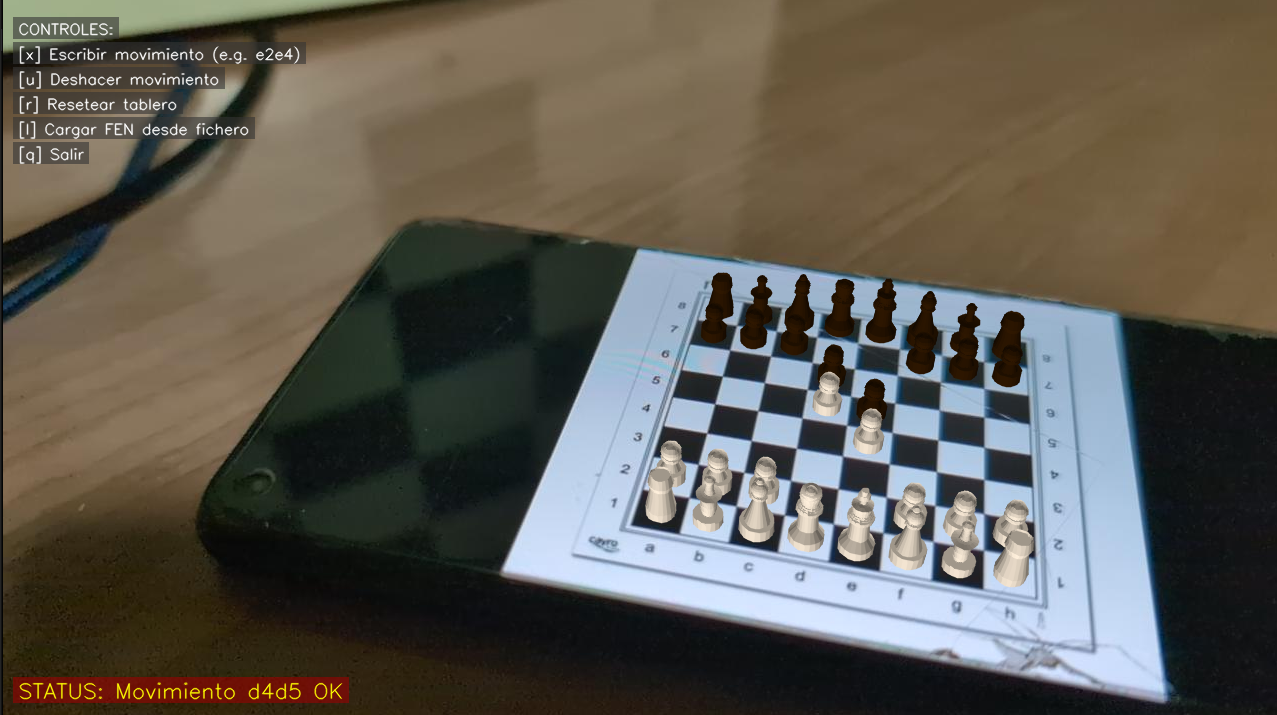
\includegraphics[width=0.8\textwidth]{images/hud_interface.png}
    \caption{Interfaz de usuario superpuesta en tiempo real, mostrando el menú de controles y el estado del juego.}
    \label{fig:hud}
\end{figure}

Como se muestra en la imagen anterior, la aplicación puede funcionar sobre cualquier objeto que contenga un patrón de tablero de ajedrez, permitiendo jugar partidas de ajedrez virtual sobre un tablero real, un cuaderno o incluso una pantalla digital. 

\subsection{Conclusiones y Trabajo Futuro}

En este bloque de trabajo se ha desarrollado con éxito un sistema completo de Realidad Aumentada monocular. Se ha demostrado que es posible lograr un renderizado 3D convincente y estable utilizando únicamente herramientas de visión por computador y cálculo matricial, sin depender de motores gráficos de alto nivel.

Los resultados muestran un rendimiento robusto ($\sim 30$ ms por frame) y una alta estabilidad geométrica gracias a los algoritmos de ordenación de esquinas implementados. 
Como líneas de trabajo futuro, se podría proponer la integración de elementos que mejoren la experiencia de usuario como animaciones,
iluminación de casillas para indicar movimientos legales o la posibilidad de interactuar físicamente con la detección de gestos de mano.

En el video adjunto se pueden observar las propiedades del sistema en tiempo real, incluyendo la detección del tablero, la proyección de las piezas, la interactividad mediante teclado y la coherencia temporal en la estimación de pose.

\clearpage

\section*{Uso de IA}

Se ha utilizado IA conversacional para asistencia en la elaboración de código,
en específico el modelo Pro de Gemini de Google. Todo el contenido generado 
fue revisado y adaptado por los autores.

\bibliographystyle{ieeetr}
\bibliography{references}

\end{document}

